\documentclass[12pt]{article}
\title{CS310 Final Report \\ The Role of Bartle's Gamer Types in Higher Education}
\author{William Seymour, Third Year Computer Science \\ Supervisor: Mike Joy}
\date{\today}
\linespread{1.3}

\usepackage{cite}
\usepackage{graphicx}
\usepackage{url}
\usepackage{fullpage}
\usepackage{verbatim}
\usepackage{microtype}

\begin{document}
\maketitle
\clearpage
\tableofcontents
\listoffigures
\listoftables

\section{Abstract}
Gamification and analytics are becoming increasingly popular in many facets of everyday life. They are making a big impact in primary and secondary education, driven by the increased use of internet enabled devices in the classroom. This project looks at how this can be translated to higher education, and what role the traditional gamification personality types might have in this field.

\section{Key words}
Gamification, Psychological profiling, Higher education, User typology

\section{Introduction}
Gamification has become an increasingly influential force in the marketing world over previous years. The benefit of integrating these techniques into primary and secondary education was clear from the onset, but there has been less enthusiasm for their use in higher education. This report will assess the usefulness of a particular method of categorising players commonly used in gamification in directing learning in the higher education sector. The main body will explore the application of the Bartle personality types used in gamification, with particular interest in how they interact with currently accepted models of personality and learner typologies like Keirsey temperaments.

The recent discovery of gamification has meant that far less has been done to incorporate developments on it into the current education system than might be possible at some future point in time. The project starts with a look at the background of gamification before progressing on to how these techniques are being integrated into the current primary and secondary education sectors successfully, as well as the differences between the those sectors and the higher education sector. Then the study undertaken to determine the link between gamer and personality types will be presented, and the results discussed.

\section{Background}
\subsection{What is Gamification?}
It seems an obvious fact of life that work is dull, and play is fun. Many attempts have been made to change this, but they have largely been met with little success. Over the past few years, gamification has been slowly blurring the lines of what is considered to be `work' by moving it towards practises and behaviours that would normally be associated with play. This has all come out of a field of study which is fairly young, the term having only really gained popularity in late 2010, as shown in figure \ref{usagegraph}. Coupled with the advanced user tracking and analytics offered by modern technology, it has begun to dominate the way in which we interact electronically, with services like Facebook and Foursquare being prime examples.

\begin{figure}[p]
	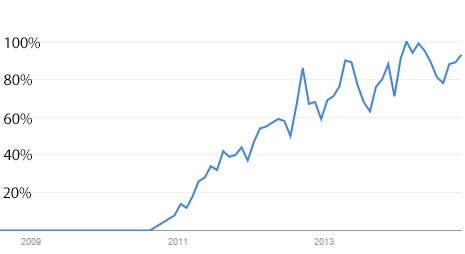
\includegraphics{../img/usage-graph.png}
	\caption{Usage of the term `gamification' by month as a proportion of the total number of Google searches for gamification, from 2009 to the present day \cite{usage}.}
	\label{usagegraph}
\end{figure}

At its core, it is the idea of taking the elements which have made traditional games provided fun and entertainment for all of human history, and using them to transform everyday tasks which many find less interesting. While the results so far of gamified experiences are very promising, with many use cases reporting exponential increases in customer attraction and retention \cite{zichermann2010game}, there are some ethical questions raised due to the fact that gamification often takes the form of operant conditioning \cite{kapp2012gamification}. While manipulating users in order to stimulate learning is often lauded as being virtuous, using it to sell products and make a profit might not. This will be explored more in section \ref{sec:issues}.

\subsection{How does it work?}
The success of gamification in driving engagement has underlying roots in psychology, with gameified experiences being able to satisfy more psychological needs than what might normally be considered `work'. For example, the feedback mechanisms which typify these experiences, such as progress bars, badges and the awarding of in-game points, help fulfil the need for competence which self determination theory identifies as a core need experienced by all human beings \cite{przybylski2010motivational}. Players are compelled to complete game actions in order to feel capable, and challenges often use time investment as the principal measure of worth. Traditional games tend to confer rewards and status based on skill, which can alienate a large proportion of the player base who fall outside the top performers. In this way all players feel as if they can succeed if they play the game for long enough, or regularly enough.

As mentioned above, a key part of the psychology behind gamification is that of operant conditioning. Introduced as a concept by B.F. Skinner, it focuses on conditioning organisms to perform tasks that they would not normally undertake. In his experiments, Skinner would place pigeons in boxes and reward them with food whenever they pushed a button in their cage. If every push of the button resulted in a reward, the birds would stop pecking as soon as the food stopped being dispensed. He found that when rewards were awarded on a semi random basis, the animals would continue to peck at the buttons long after the food was gone \cite{kapp2012gamification}. This form of conditioning is used to great effect in many forms of gambling, and is the reason gamblers will continue to insert coins into machines in the hope that they might get that elusive win. Indeed, it seems counterintuitive that reducing the frequency of rewards might actually increase uptake by users. It turns out that chasing a win or payoff with slim odds is for more exciting than completing an action with a known reward. In fact, it may well be that the act of achieving a rare reward is motivation in itself, even if there is no real world value attached to it. Thus operant conditioning is used to keep users playing even after the activity has ceased to be fun.

\subsection{High profile usages of gamification}
As gamification expands more and more into everyday life, each sector is asking the question of how they can keep up. To a certain extent, a change of thinking is required. Increasingly it is becoming a question of why should people be expected to stop having fun in order to learn, watch an advertisement or communicate? \cite{zichermann2010game} Or, put more bluntly, why would they? The rise of gamification has meant that other forms of experience are less effective than they once were, just by virtue of the new competition. What follows are a pair of case studies of gamification employed by high profile organisations to serve as a practical example of what exactly gamification and analytics mean in the context of the modern day, and proof of how effective they can be when used to their full potential.

\subsubsection{Case Study: Orkut}

An early example of the power of gamification can be seen in Orkut, the social networking site which was developed by Google in early 2004. Orkut was different from other social networks available at the time in that users had profiles operating on three different levels. Information provided by users was divided up into personal, professional and social, with the aim of having users connect on different levels. More interestingly in terms of gamification, Orkut would provide a real time list of demographics about the current user population \cite{fragoso2006wtf}. It was one such demographic, usage by country, that began a completely unexpected phenomenon in Brazil. In an attempt to climb to the top of what many began to perceive as a leaderboard, blogs and social media posts started appearing all over Brazilian internet sites urging others to join \cite{zichermann2010game}. By June 2004 the number of Brazilian users had surpassed those from the United States to take the top spot on the usage demographics, and went on to continue climbing rapidly. What had begun as an interesting statistic had motivated thousands of people to become invested in a product to such an extent that Orkut's domination of the Brazilian social network scene did not end until December 2012 when Facebook finally wrested the crown from the Google network \cite{1_comscore_2012}. It is important to note that the engagement driven by gamification was long lasting: Orkut continued to be dominated by Brazilian users even though the initial challenge had ended. Persistent usage over localised surges is key to successful analysis of gamification applications.

\begin{figure}[p]
	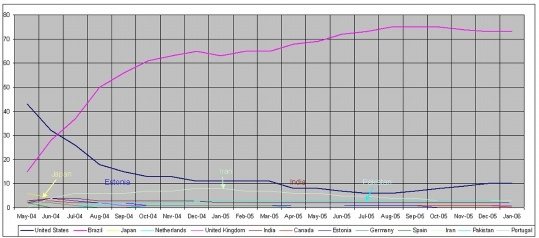
\includegraphics{../img/orkut-brazil.jpg}
	\caption{Orkut usage by country, shown for the top ten nations among the user population. Data from May 2004 to January 2006 \cite{fragoso2006wtf}.}
	\label{orkut-brazil}
\end{figure}

\subsubsection{Case Study: Frequent Flyer Programs}
Since their introduction by airlines in the 1980s, frequent flyer programs have become incredibly popular. What makes them interesting from a gamification perspective is the degree of long term loyalty and engagement they inspire in their users. It is not unheard of for customers to take flight options that are longer and less efficient, or indeed entirely superfluous, with the sole intent of accruing extra air miles with their chosen carrier. They skilfully employ various game elements in order to persuade customers to keep coming back time and again. The giving of status is ubiquitous among frequent flyer programs, and is something that many are keen to chase. In fact, given that the number of air miles being redeemed is not growing at the same rate as air mile acquisition, as shown in figure \ref{freq-flyer}, it could be suggested that for many, status is in fact the end goal and not the means as one might at first assume. Zichermann and Linder even go as far as to directly compare such programs to massively multiplayer online games, pointing out the similarity between experience points leading to an increase in level and air miles leading to an increase in status. From the perspective of an involved airline, loyalty schemes are very good for business. Most of the rewards conferred by elite status in a frequent flyer program, such as an airline lounge or expedited boarding, require little or no money to be spent on the part of an airline. More recently, the impact of air miles schemes has expanded to influence almost all parts of everyday life, with points commonly being offered for airline branded credit cards and bookings at partnered hotels. This has all resulted in frequent flyer programs becoming the leading revenue stream for many airlines, reporting higher profits and creating entire virtual economies \cite{zichermann2010game}.

\begin{figure}[p]
	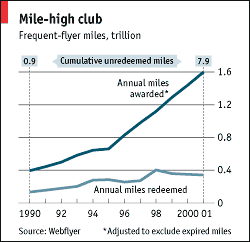
\includegraphics{../img/flyer.png}
	\caption{Total air miles rewarded and redeemed from 1990 to 2001 \cite{freq-fly}.}
	\label{freq-flyer}
\end{figure}

\section{Definitions}
Before continuing it is important to define some of the key terms that will be used in this report. Words like gamification and analytics are often bandied around by lots of different parties who all mean similar but subtly different things. Indeed, the way in which these terms have been used thus far has been somewhat vague. For the remainder of the document, the undermentioned should be referred to as a definitive explanation of what is meant by the following technical terms.

\subsection{Gamification}
A commonly accepted definition of gamification put forward by Detarding, et al. \cite{deterding2011game} and supported by Manrique \cite{iversitymooc} is that it is (broadly) ``the use of game design elements in non-game contexts''. This is a good explanation in that it makes clear the distinction between games and gamified activities, but what exactly counts as either can often be left unclear. This is difficult as it is near impossible to pin down where one stops and the other begins, and this problem is likely to increase as game elements are further incorporated into everyday activities. Indeed, this seems to suggest that rigorously defining what is and is not a game is of less value than originally anticipated. Here, a game is best held to refer to experiences that are labelled as games. While this might seem self evident, the majority of the gamified experiences from which we wish to differentiate them do not label themselves as games. It follows that a non game context is often one in which the users have little or no understanding that they are participating in a game, often because they are passively playing, whereas games as defined above generally require more active involvement.

Game elements also need to be outlined in a little more depth. For the purposes of this project, they will be taken to mean those elements of game systems which compel users to play because they are engaging or fun. Alternatively put, the focus is on the mechanics that make games interesting and keep users coming back as opposed to graphical techniques or the platforms they reside on. The reasoning for this is that these features are not easily ported to other contexts and the ones in which they are shared are of no relevance to the report. If a non game context begins to feature such things as controller support or complex 3D rendering, one would be hard pressed to justify it as such. For the latter point mentioned above, films are a good example of a field which shares many elements with the graphical techniques employed by modern games but has nothing inherently to do with gamification.

\subsection{Analytics}
The other component to the project is analytics, with a focus on online learning platforms. In this context analytics refers to feedback systems which collect data on various facets of the learning process. Crucially, they must provide information which can then be used to improve the process further and better understand the dynamics of class makeup and teaching styles, under analysis by either the system itself or a human analyst. This is to provide some differentiation from software which merely reports back statistics such as student or class scores, with no extra dimension by which the effectiveness of the setup as a whole can be bettered. It does not matter if some of the data is collected offline.

Tracking and comparing different sets of statistics in this way shows correlations that might otherwise be missed. Singling out these links is the key to effective improvement of higher education. It is not required for the purposes of this definition that the analysis be automated and carried out by the system itself. In many small scale implementations, such as the one used for this project, the resources available preclude the development of such an advanced piece of software. Indeed, implementing a prototype smart learning platform would be too expensive for many institutions, and excluding them would have a negative impact on the data that could be obtained.

\subsection{Gamer and Personality Types}
Throughout the report many references will be made to gamer and personality types. It is important to note that these metrics are not the same, and that they are not necessarily equivalent in any way. Gamer type will be used to refer to the four player types, Achiever, Explorer, Killer and Socialiser, identified by Bartle \cite{bartle1996hearts}, used to categorise the way in which players behave in games. Personality types will be used to refer to either the 16 personality types or the resulting four temperaments identified by Keirsey and Bates \cite{keirsey1984} which are used to group people according to the ways in which they think and act.

\section{Literature Review}
Before continuing it is important to undertake a review of previous and current literature in the field, in order to properly frame the underwritten findings and analysis. This will begin by broadly assessing past research in the field of gamification as a whole before moving on to the more specific field of higher education. Also included will be an assessment of papers relating to Bartle's gamer types and how they might be linked with learning styles.

\subsection{Games and Gamification}
Scholars have been writing about games and their relationship with sociology for centuries, and this review will begin by examining Man, Play and Games by Caillois \cite{caillois1961man}. Caillois begins by attempting to pin down what exactly he means by a game, and how they can be classified. He concurs with the view expressed above in that this is a difficult task given the wide diversity of games. While most of the book focuses on more traditional games and forms of play, of particular interest is the chapter on the corruption of games in the then modern world. By beginning to draw parallels between the behaviours exhibited in games and the behaviours exhibited in real life, his work can help us to understand which areas of our subject matter might be more easily gamified, and the potential pitfalls we should aim to avoid if this is not done with a due amount of care. While this may seem a little extreme at first glance, the stories of addiction resulting from various online multiplayer and mobile games are enough to warrant more care being taken to monitor the situation than otherwise might be the case. While the examples he presents with regards to the engaging nature of games are often quite antiquated, it does serve to show how little the underlying relationship between humans and games has changed. While the manifestations of agon, alea, mimicry and ilinix have changed markedly over the last fifty years, they still very much exist today. Table \ref{table:corruption} shows the relationships Caillois claims exists between play types and where they can be found.

\begin{table}[p]
	\begin{tabular}{|p{2.0cm}|p{4.2cm}|p{4.2cm}|p{4.2cm}|}
		\hline - & Cultural Forms & Institutional Forms & Corruption \\ 
		\hline AGON (Compettition) & Sports & Economic compettion and competitive examinations & Violence, Will to power and Trickery \\ 
		\hline ALEA (Chance) & Lotteries and Casinos & Speculation on the stock market & Superstition, astrology, etc. \\ 
		\hline MIMICRY (Simulation) & Carnival, Theatre, Cinema and Hero worship & Uniforms and Ceremonial etiquette & Alienation and Split personality \\ 
		\hline ILINX (Vertigo) & Mountain climbing, Skiing, Tightrope walking and Speed & Professions requiring control of vertigo & Alcoholism and Drugs \\ 
		\hline 
	\end{tabular}
	\caption{Caillois's mapping of play types to social life \cite{caillois1961man}. In this context, vertigo refers to ``an attempt to momentarily destroy the stability of perception and inflict a kind of voluptuous panic upon an otherwise lucid mind''.}
	\label{table:corruption}
\end{table}

A more modern interpretation on what makes games, specifically digital games, engaging is offered by Schoenau-Fog \cite{schoenau2011player}. By presenting a survey on what drives the `continuation desire' in players, that is to say the desire they have to pursue the continuation of a game experience, it is possible to better understand what compels the modern game user. The results of the questionnaire can be seen in figure \ref{fog}. Understanding the engagement categories is key to the creation of effective gamified experiences, and it is interesting to see how they fit in with the play types identified by Callois \cite{caillois1961man}. These categories have a strong basis in psychology, and mesh well with the values of autonomy, competence and relatedness purported by self determination theory that Sheldon and Filak have shown to be unique and basic human psychological needs \cite{sheldon2008manipulating}. However, the Objectives, Activity, Accomplishment and Affect framework Schoenau puts forward is not very rigorous. Though it is informed by analysis of the survey responses it adds little to the way that people interact with games, and its only real use is as a basis for the player engagement process later on in the paper.

\begin{figure}[p]
	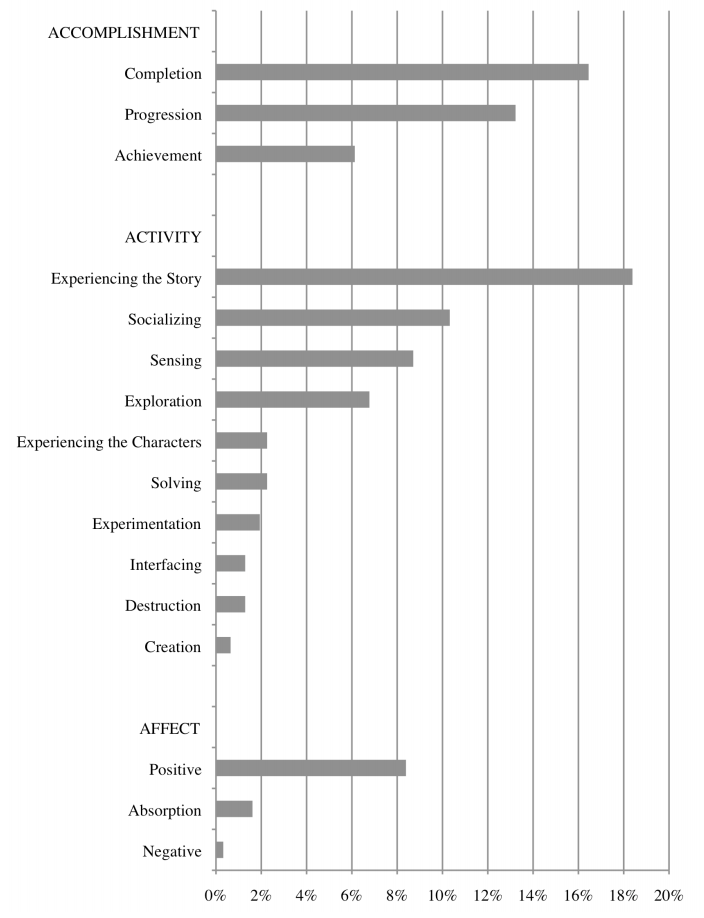
\includegraphics[width=0.75\textwidth]{../img/fog.png}
	\caption{Categories of player engagement rank-ordered: ``What in a game makes you want to continue playing?'' \cite{schoenau2011player}.}
	\label{fog}
\end{figure}

No study relating to gamification would be complete without an assessment of `Hearts, clubs, diamonds, spades: Players who suit MUDs' b Richard Bartle \cite{bartle1996hearts}. Written in 1996 it introduced the first real model of gamer personality types, shown in table \ref{table:cards}, which allow players to be grouped based on the habits and tenancies they exhibit while playing games. Such a model allows users to catered for according to their preferences, as well as allowing game designers to take a more rigorous approach to balancing the behaviours seen in their games.  One weakness in the paper which Bartle himself acknowledges is that in not being qualified as a psychologist he is unable to provide an in-depth scientific background to his findings. While the paper lays the groundwork for classifying users by their observed behaviours in-game, its approach is not very granular, and can often be quite a blunt way of grouping people. Bartle did expand this model in his 2005 paper, Virtual Worlds: Why People Play, but this was partly to address the changing of players over time, and the only extra distinctions offered are explicit (acting first) and implicit (thinking first) variants of the four presented in the aforementioned 1996 paper \cite{bartle2005play}. That said, his work has formed the basis for how many identify the ways in which people play games, and has been very influential in the design of gameified systems.

\begin{table}[p]
\begin{tabular}{|c|c|c|}
	\hline - & Acting & Interacting \\ 
	\hline Players & Killers & Socialisers \\ 
	\hline World & Achievers & Explorers \\ 
	\hline 
\end{tabular}
\caption{Bartle's four gamer types \cite{bartle1996hearts}.}
\label{table:cards}
\end{table}

[Gamification of higher education]

\subsection{Higher Education}

\section{Gamified Primary and Secondary Education}

\section{How Higher Education is Different}

\section{Bartle's Gamer Types}

\section{Focus Group}

\subsection{Methodology}

\subsection{Findings}

\subsection{Evaluation}

\section{Conclusion and Further Work}

\section{Legal, Social, Ethical and Professional Issues}
\label{sec:issues}

\section{Background Texts}
[Please understand me]

\section{Appendicies}
\subsection{Appendix I: Bartle Test Questions}
As written by Erwin Andreasen and Brandon Downey. Retrieved from \url{http://www.andreasen.org/bartle/questions-en.dat} on 22/01/2015.
\linespread{1.0}
\begin{verbatim}
Are you more comfortable, as a player on a MUD:
+S Talking with friends in a tavern?
+A Out hunting orcs by yourself for experience?

Which is more enjoyable to you?
+A Killing a big monster
+S Bragging about it to your friends?

Which do you enjoy more in MUD quests:
+S Getting involved in the storyline
+A Getting the rewards at the end?

Which would you rather be noticed for on a MUD?:
+A Your equipment
+S Your personality

Would you rather be:
+S Popular
+A Wealthy

Which do you enjoy more on a MUD?:
+S Getting the latest gossip
+A Getting a new item

Which would you enjoy more as a MUD player?
+S Running your own tavern?
+E Making your own maps of the world, then selling them?

What's more important in a MUD to you?
+S The number of people
+E The number of areas to explore

What's more important to you:
+S The quality of roleplaying in a MUD
+E The uniqueness of the features and game mechanic

You are being chased by a monster on a MUD.
Do you:
+S Ask a friend for help in killing it
+E Hide somewhere you know the monster won't follow

You're a player on a mud, and you want to fight a really tough dragon.
How would you approach this problem?
+S Get a big group of players to kill it.
+E Try a variety of weapons and magic against it, until you find its weakness.

You're a player on a MUD, and about to go into an unknown dungeon.
You have your choice of one more person for your party.
Do you bring:
+S A bard, who's a good friend of yours and who's great for entertaining you 
and your friends
+E A wizard, to identify the items that you find there

Is it better to be:
+K Feared
+S Loved

Someone has PK'ed you. Do you want to:
+S Find out why, and try to convince them not to do it again
+K Plot your revenge

Which is more exciting?
+S A well-roleplayed scenario
+K A deadly battle

Which would you enjoy more?
+K Winning a duel with another player
+S Getting accepted by a clan

Would you rather
+K Vanquish your enemies
+S Convince your enemies to work for you, not against you

What's worse:
+K To be without power
+S To be without friends

On a MUD, a new area opens up.
Which do you look forward to more?
+E Exploring the new area, and finding out its history
+A Being the first to get the new equipment from the area

On a MUD, would you rather be known as:
+E Someone who can run from any two points in the world, and really knows
their way around.
+A The person with the best, most unique equipment in the game

Would you rather:
+A Become a hero faster than your friends
+E Know more secrets than your friends?

Would you rather:
+E Know where to find things
+A Know how to get things?

Which would you rather do:
+E Solve a riddle no one else has gotten
+A Getting to a certain experience level faster than anyone else

Do you tend to:
+E Know things no one else does
+A Have items no one else does

On a MUD, would rather join a clan of:
+E Scholars
+K Assassins

Would you rather win:
+E A trivia contest
+K An arena battle

If you're alone in an area, do you think:
+E It's safe to explore
+K You'll have to look elsewhere for prey

On a MUD, would rather be known for
+E Knowledge
+K Power

Would you rather:
+K Defeat an enemy
+E Explore a new area

You learn that another player is planning your demise.
Do you:
+E Go to an area your opponent is unfamiliar with and prepare there
+K Attack him before he attacks you

On a MUD, would you rather:
+A Have a sword twice as powerful as any other in the game
+K Be the most feared person in the game

On a MUD, would you be more prone to brag about:
+K How may other players you've killed
+A Your equipment

Would you rather have:
+K A spell to damage other players
+A A spell that increases the rate at which you gain experience points?

Would you rather have:
+A Two levels of experience
+K An amulet that increases the damage you do against other players by 10%.

Would you rather receive as a quest reward:
+A Experience points
+K A wand with 3 charges of a spell that lets you control other players,
against their will. (charm person)

When playing a video game, is it more fun to:
+A Have the highest score on the list?
+K Beat your best friend one-on-one?
\end{verbatim}
\linespread{1.3}

\bibliography{references}
\bibliographystyle{plain}
\end{document}